\documentclass{article}\usepackage[]{graphicx}\usepackage[]{color}
%% maxwidth is the original width if it is less than linewidth
%% otherwise use linewidth (to make sure the graphics do not exceed the margin)
\makeatletter
\def\maxwidth{ %
  \ifdim\Gin@nat@width>\linewidth
    \linewidth
  \else
    \Gin@nat@width
  \fi
}
\makeatother

\definecolor{fgcolor}{rgb}{0.345, 0.345, 0.345}
\newcommand{\hlnum}[1]{\textcolor[rgb]{0.686,0.059,0.569}{#1}}%
\newcommand{\hlstr}[1]{\textcolor[rgb]{0.192,0.494,0.8}{#1}}%
\newcommand{\hlcom}[1]{\textcolor[rgb]{0.678,0.584,0.686}{\textit{#1}}}%
\newcommand{\hlopt}[1]{\textcolor[rgb]{0,0,0}{#1}}%
\newcommand{\hlstd}[1]{\textcolor[rgb]{0.345,0.345,0.345}{#1}}%
\newcommand{\hlkwa}[1]{\textcolor[rgb]{0.161,0.373,0.58}{\textbf{#1}}}%
\newcommand{\hlkwb}[1]{\textcolor[rgb]{0.69,0.353,0.396}{#1}}%
\newcommand{\hlkwc}[1]{\textcolor[rgb]{0.333,0.667,0.333}{#1}}%
\newcommand{\hlkwd}[1]{\textcolor[rgb]{0.737,0.353,0.396}{\textbf{#1}}}%
\let\hlipl\hlkwb

\usepackage{framed}
\makeatletter
\newenvironment{kframe}{%
 \def\at@end@of@kframe{}%
 \ifinner\ifhmode%
  \def\at@end@of@kframe{\end{minipage}}%
  \begin{minipage}{\columnwidth}%
 \fi\fi%
 \def\FrameCommand##1{\hskip\@totalleftmargin \hskip-\fboxsep
 \colorbox{shadecolor}{##1}\hskip-\fboxsep
     % There is no \\@totalrightmargin, so:
     \hskip-\linewidth \hskip-\@totalleftmargin \hskip\columnwidth}%
 \MakeFramed {\advance\hsize-\width
   \@totalleftmargin\z@ \linewidth\hsize
   \@setminipage}}%
 {\par\unskip\endMakeFramed%
 \at@end@of@kframe}
\makeatother

\definecolor{shadecolor}{rgb}{.97, .97, .97}
\definecolor{messagecolor}{rgb}{0, 0, 0}
\definecolor{warningcolor}{rgb}{1, 0, 1}
\definecolor{errorcolor}{rgb}{1, 0, 0}
\newenvironment{knitrout}{}{} % an empty environment to be redefined in TeX

\usepackage{alltt}

% \usepackage[utf8]{inputenc}
\usepackage{amsmath}
\usepackage{fancyhdr}
\usepackage{array}
\usepackage{longtable}
\usepackage{graphicx}
\usepackage{color}
\usepackage[letterpaper, margin=1in]{geometry}
\usepackage{lscape}
\newcommand{\blandscape}{\begin{landscape}}
\newcommand{\elandscape}{\end{landscape}}
\usepackage{dcolumn}
\usepackage{bbm}
\usepackage{threeparttable}
\usepackage{booktabs}
\usepackage{expex}
\usepackage{pdflscape}
\usepackage{rotating, graphicx}
\usepackage{tabulary}
\usepackage{lscape}
\usepackage{makecell}
\usepackage{algorithm}
\usepackage{multirow}
\usepackage{colortbl}
\usepackage{longtable}
\usepackage{array}
\usepackage{multirow}
\usepackage{wrapfig}
\usepackage{float}
\usepackage{pdflscape}
\usepackage{tabu}
\usepackage{threeparttable}

\title{%
Homework 3\\
\large Applied Mutlivariate Analysis}
\date{September 22, 2018}
\author{Emorie Beck}
\IfFileExists{upquote.sty}{\usepackage{upquote}}{}
\begin{document}
\maketitle
% \SweaveOpts{concordance=TRUE}

\section{Workspace}
\subsection{Packages}



\begin{knitrout}
\definecolor{shadecolor}{rgb}{0.969, 0.969, 0.969}\color{fgcolor}\begin{kframe}
\begin{alltt}
\hlkwd{library}\hlstd{(car)}
\hlkwd{library}\hlstd{(knitr)}
\hlkwd{library}\hlstd{(psych)}
\hlkwd{library}\hlstd{(kableExtra)}
\hlkwd{library}\hlstd{(multcomp)}
\hlkwd{library}\hlstd{(lme4)}
\hlkwd{library}\hlstd{(plyr)}
\hlkwd{library}\hlstd{(tidyverse)}
\hlkwd{library}\hlstd{(MVN)}
\end{alltt}
\end{kframe}
\end{knitrout}



\subsection{data}
The file, Set\_5.csv, contains data from a study in which college students completed the NEO-PI Personality Inventory. This 240-item scale purportedly measures the Big Five personality dimensions, assumed to be fairly independent. The inventory is scored on 6 subscales per dimension, listed below. The file contains the subscale scores, rather than the individual items, which should help reduce the impact of the small sample size.\\

Neuroticism: Anxiety
Neuroticism: Angry\_Hostility
Neuroticism: Depression
Neuroticism: Self\_Consciousness
Neuroticism: Impulsiveness
Neuroticism: Vulnerability
Extraversion: Warmth
Extraversion: Gregariousness
Extraversion: Assertiveness
Extraversion: Activity
Extraversion: Excitement\_Seeking
Extraversion: Positive\_Emotions
Openness: Fantasy
Openness: Aesthetics
Openness: Feelings
Openness: Actions
Openness: Ideas
Openness: Values
Agreeableness: Trust
Agreeableness: Straightforwardness 
Agreeableness: Altruism
Agreeableness: Compliance
Agreeableness: Modesty
Agreeableness: Tender\_Mindedness
Conscientiousness: Competence
Conscientiousness: Order
Conscientiousness: Dutifulness
Conscientiousness: Achievement\_Striving: 
Conscientiousness: Self\_Discipline
Conscientiousness: Deliberation

\begin{knitrout}
\definecolor{shadecolor}{rgb}{0.969, 0.969, 0.969}\color{fgcolor}\begin{kframe}
\begin{alltt}
\hlstd{wd} \hlkwb{<-} \hlstr{"https://github.com/emoriebeck/homeworks/raw/master/multivariate/homeworks/homework5"}

\hlstd{dat} \hlkwb{<-} \hlkwd{sprintf}\hlstd{(}\hlstr{"%s/Set_5(2).csv"}\hlstd{, wd)} \hlopt
  \hlkwd{read.csv}\hlstd{(.,} \hlkwc{stringsAsFactors} \hlstd{= F)}

\hlkwd{head}\hlstd{(dat)}
\end{alltt}
\begin{verbatim}
##   ID Anxiety Angry_Hostility Depression Self_Consciousness Impulsiveness
## 1  2   2.625           2.000      1.750           2.250000         2.625
## 2  3   3.625           2.875      3.000           3.500000         4.250
## 3  4   3.000           2.750      2.625           2.875000         3.000
## 4  5   4.375           3.125      4.500           4.000000         3.875
## 5  6   3.500           2.875      3.000           2.571429         3.625
## 6  7   4.000           4.125      2.875           2.375000         4.000
##   Vulnerability   Warmth Gregariousness Assertiveness Activity
## 1      2.166667 4.666667          4.000      3.000000 4.833333
## 2      2.125000 4.500000          2.750      2.625000 3.000000
## 3      2.875000 3.750000          3.125      2.375000 3.250000
## 4      3.750000 3.250000          2.250      2.500000 1.875000
## 5      2.750000 3.750000          3.125      3.285714 3.500000
## 6      3.125000 3.500000          2.625      3.375000 3.125000
##   Excitement_Seeking Positive_Emotions  Fantasy Aesthetics Feelings
## 1              3.500             4.750 3.857143   3.571429 4.666667
## 2              2.875             3.500 3.500000   4.125000 3.625000
## 3              3.875             3.375 3.375000   3.500000 3.250000
## 4              2.750             2.625 3.000000   3.750000 4.250000
## 5              3.750             3.625 3.125000   1.625000 3.125000
## 6              2.000             3.375 3.500000   2.000000 3.250000
##    Actions Ideas Values Trust Straightforwardness Altruism Compliance
## 1 2.571429 4.400  4.600 5.000            2.166667 4.833333      2.750
## 2 3.000000 3.875  3.125 3.250            3.750000 3.625000      3.125
## 3 2.375000 4.125  3.500 3.250            3.125000 4.000000      3.750
## 4 3.375000 2.750  4.125 3.000            3.428571 3.875000      4.000
## 5 2.750000 2.500  3.625 3.375            3.250000 4.125000      3.625
## 6 2.625000 1.125  3.625 2.500            2.875000 3.000000      2.250
##   Modesty Tender_Mindedness Competence Order Dutifulness
## 1   4.000          3.833333       4.50 3.625    3.285714
## 2   2.625          3.250000       3.00 2.250    3.875000
## 3   2.750          3.250000       3.75 3.250    3.750000
## 4   4.125          3.750000       2.75 3.000    2.875000
## 5   3.375          3.375000       3.75 4.000    3.750000
## 6   2.625          3.375000       3.00 3.625    2.625000
##   Achievement_Striving Self_Discipline Deliberation
## 1             4.333333           4.250        2.875
## 2             2.750000           3.750        3.500
## 3             3.375000           3.375        3.125
## 4             2.875000           2.625        3.250
## 5             3.375000           2.875        3.375
## 6             3.000000           2.625        2.625
\end{verbatim}
\end{kframe}
\end{knitrout}

\begin{knitrout}
\definecolor{shadecolor}{rgb}{0.969, 0.969, 0.969}\color{fgcolor}\begin{kframe}
\begin{alltt}
\hlstd{source} \hlkwb{<-} \hlkwd{tribble}\hlstd{(}
\hlopt{~}\hlstd{Factor,} \hlopt{~}\hlstd{Facet,}
\hlstr{"Neuroticism"}\hlstd{,} \hlstr{"Anxiety"}\hlstd{,}
\hlstr{"Neuroticism"}\hlstd{,} \hlstr{"Angry_Hostility"}\hlstd{,}
\hlstr{"Neuroticism"}\hlstd{,} \hlstr{"Depression"}\hlstd{,}
\hlstr{"Neuroticism"}\hlstd{,} \hlstr{"Self_Consciousness"}\hlstd{,}
\hlstr{"Neuroticism"}\hlstd{,} \hlstr{"Impulsiveness"}\hlstd{,}
\hlstr{"Neuroticism"}\hlstd{,} \hlstr{"Vulnerability"}\hlstd{,}
\hlstr{"Extraversion"}\hlstd{,} \hlstr{"Warmth"}\hlstd{,}
\hlstr{"Extraversion"}\hlstd{,} \hlstr{"Gregariousness"}\hlstd{,}
\hlstr{"Extraversion"}\hlstd{,} \hlstr{"Assertiveness"}\hlstd{,}
\hlstr{"Extraversion"}\hlstd{,} \hlstr{"Activity"}\hlstd{,}
\hlstr{"Extraversion"}\hlstd{,} \hlstr{"Excitement_Seeking"}\hlstd{,}
\hlstr{"Extraversion"}\hlstd{,} \hlstr{"Positive_Emotions"}\hlstd{,}
\hlstr{"Openness"}\hlstd{,} \hlstr{"Fantasy"}\hlstd{,}
\hlstr{"Openness"}\hlstd{,} \hlstr{"Aesthetics"}\hlstd{,}
\hlstr{"Openness"}\hlstd{,} \hlstr{"Feelings"}\hlstd{,}
\hlstr{"Openness"}\hlstd{,} \hlstr{"Actions"}\hlstd{,}
\hlstr{"Openness"}\hlstd{,} \hlstr{"Ideas"}\hlstd{,}
\hlstr{"Openness"}\hlstd{,} \hlstr{"Values"}\hlstd{,}
\hlstr{"Agreeableness"}\hlstd{,} \hlstr{"Trust"}\hlstd{,}
\hlstr{"Agreeableness"}\hlstd{,} \hlstr{"Straightforwardness"} \hlstd{,}
\hlstr{"Agreeableness"}\hlstd{,} \hlstr{"Altruism"}\hlstd{,}
\hlstr{"Agreeableness"}\hlstd{,} \hlstr{"Compliance"}\hlstd{,}
\hlstr{"Agreeableness"}\hlstd{,} \hlstr{"Modesty"}\hlstd{,}
\hlstr{"Agreeableness"}\hlstd{,} \hlstr{"Tender_Mindedness"}\hlstd{,}
\hlstr{"Conscientiousness"}\hlstd{,} \hlstr{"Competence"}\hlstd{,}
\hlstr{"Conscientiousness"}\hlstd{,} \hlstr{"Order"}\hlstd{,}
\hlstr{"Conscientiousness"}\hlstd{,} \hlstr{"Dutifulness"}\hlstd{,}
\hlstr{"Conscientiousness"}\hlstd{,} \hlstr{"Achievement_Striving"}\hlstd{,}
\hlstr{"Conscientiousness"}\hlstd{,} \hlstr{"Self_Discipline"}\hlstd{,}
\hlstr{"Conscientiousness"}\hlstd{,} \hlstr{"Deliberation"}
\hlstd{)}

\hlstd{dat} \hlkwb{<-} \hlstd{dat} \hlopt \hlkwd{select}\hlstd{(ID, source}\hlopt{$}\hlstd{Facet)}
\end{alltt}
\end{kframe}
\end{knitrout}



\section{The Question}
Given what you have learned up through exploratory factor analysis, analyze the data in the way you think is appropriate and form conclusions about the claimed number of dimensions and their independence.

\subsection{Check for Outliers}
\begin{knitrout}
\definecolor{shadecolor}{rgb}{0.969, 0.969, 0.969}\color{fgcolor}\begin{kframe}
\begin{alltt}
\hlstd{dat2} \hlkwb{<-} \hlstd{dat} \hlopt \hlkwd{select}\hlstd{(}\hlopt{-}\hlstd{ID)} \hlopt \hlstd{data.frame}
\hlkwd{rownames}\hlstd{(dat2)} \hlkwb{<-} \hlstd{dat}\hlopt{$}\hlstd{ID} \hlcom{#1:nrow(dat2)}
\hlstd{(mv} \hlkwb{<-} \hlkwd{mvn}\hlstd{(dat2,}\hlkwc{mvnTest}\hlstd{=}\hlstr{"mardia"}\hlstd{,} \hlkwc{multivariatePlot}\hlstd{=}\hlstr{"qq"}\hlstd{,}\hlkwc{multivariateOutlierMethod}\hlstd{=}\hlstr{"quan"}\hlstd{,}\hlkwc{showOutliers}\hlstd{=}\hlnum{TRUE}\hlstd{))}
\end{alltt}
\end{kframe}
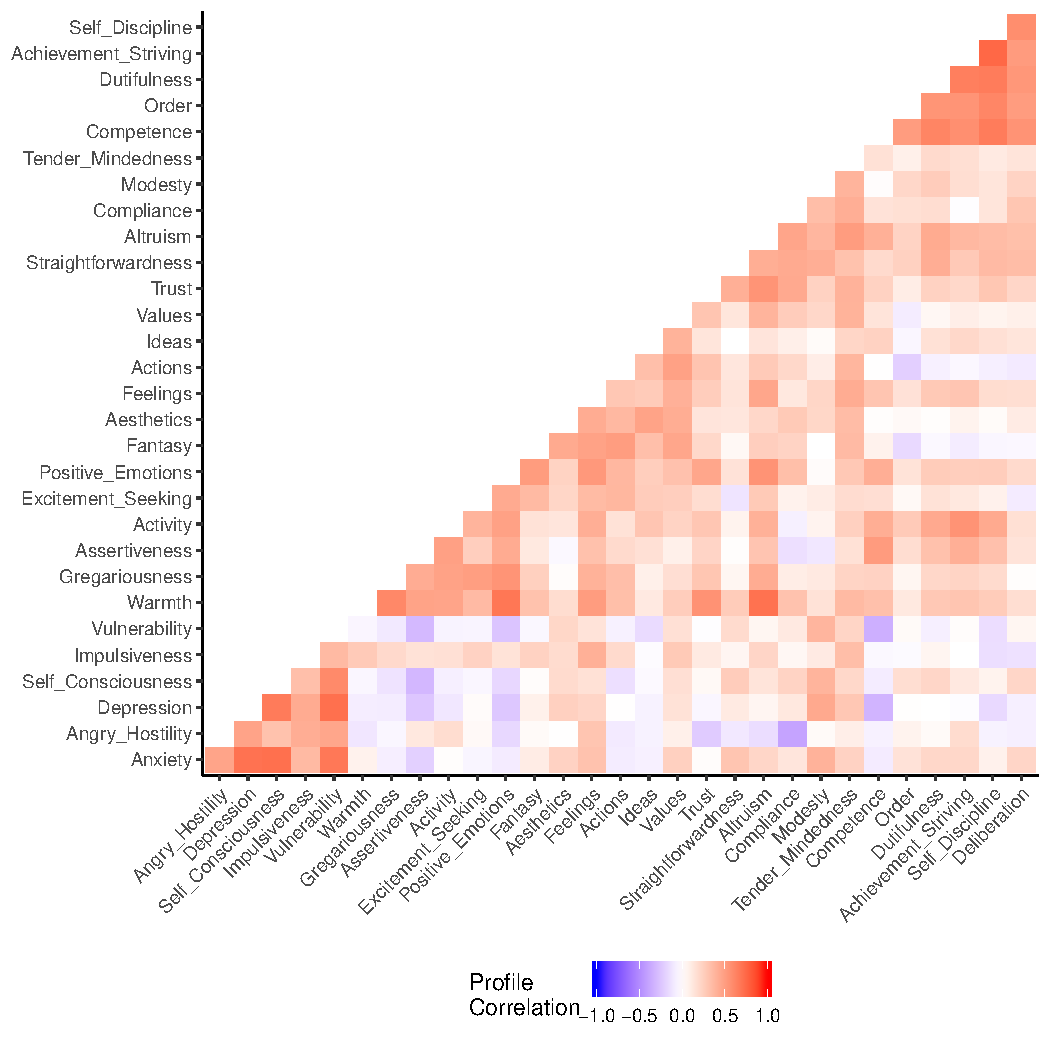
\includegraphics[width=\maxwidth]{figure/unnamed-chunk-5-1} 

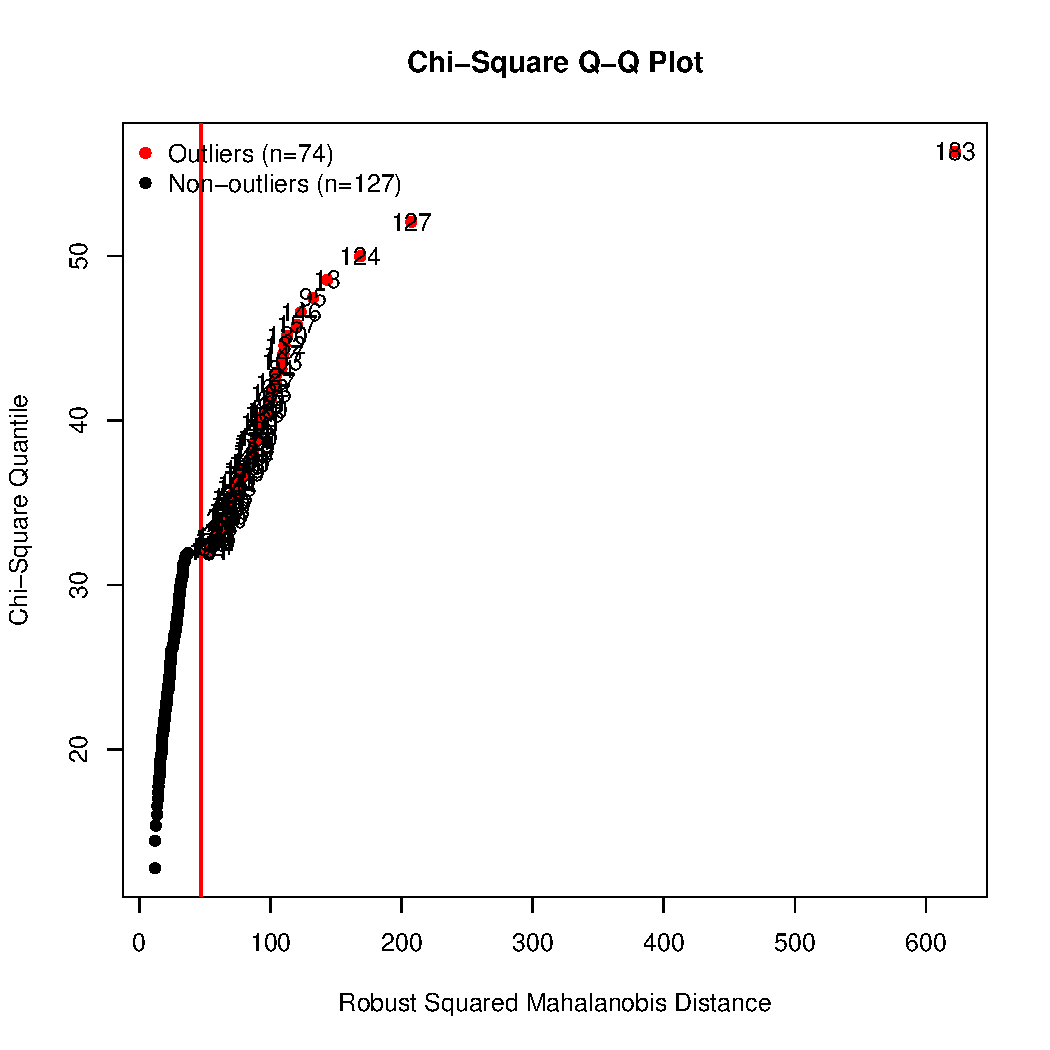
\includegraphics[width=\maxwidth]{figure/unnamed-chunk-5-2} 
\begin{kframe}\begin{verbatim}
## $multivariateNormality
##              Test        Statistic               p value Result
## 1 Mardia Skewness  8953.5001026237 9.27843696584267e-234     NO
## 2 Mardia Kurtosis 25.6787714020441                     0     NO
## 3             MVN             <NA>                  <NA>     NO
## 
## $univariateNormality
##            Test             Variable Statistic   p value Normality
## 1  Shapiro-Wilk       Anxiety           0.9688   2e-04      NO    
## 2  Shapiro-Wilk   Angry_Hostility       0.9826  0.0138      NO    
## 3  Shapiro-Wilk      Depression         0.9869  0.0595      YES   
## 4  Shapiro-Wilk  Self_Consciousness     0.9777  0.0028      NO    
## 5  Shapiro-Wilk    Impulsiveness        0.9472  <0.001      NO    
## 6  Shapiro-Wilk    Vulnerability        0.9857  0.0391      NO    
## 7  Shapiro-Wilk        Warmth           0.9344  <0.001      NO    
## 8  Shapiro-Wilk    Gregariousness       0.9785  0.0036      NO    
## 9  Shapiro-Wilk    Assertiveness        0.9839  0.0211      NO    
## 10 Shapiro-Wilk       Activity          0.9547  <0.001      NO    
## 11 Shapiro-Wilk  Excitement_Seeking     0.9499  <0.001      NO    
## 12 Shapiro-Wilk  Positive_Emotions      0.9491  <0.001      NO    
## 13 Shapiro-Wilk       Fantasy           0.9523  <0.001      NO    
## 14 Shapiro-Wilk      Aesthetics         0.9735   7e-04      NO    
## 15 Shapiro-Wilk       Feelings          0.9154  <0.001      NO    
## 16 Shapiro-Wilk       Actions           0.9627  <0.001      NO    
## 17 Shapiro-Wilk        Ideas            0.9696   2e-04      NO    
## 18 Shapiro-Wilk        Values           0.9087  <0.001      NO    
## 19 Shapiro-Wilk        Trust            0.9527  <0.001      NO    
## 20 Shapiro-Wilk Straightforwardness     0.9687   2e-04      NO    
## 21 Shapiro-Wilk       Altruism          0.9090  <0.001      NO    
## 22 Shapiro-Wilk      Compliance         0.9673   1e-04      NO    
## 23 Shapiro-Wilk       Modesty           0.9718   5e-04      NO    
## 24 Shapiro-Wilk  Tender_Mindedness      0.9164  <0.001      NO    
## 25 Shapiro-Wilk      Competence         0.9493  <0.001      NO    
## 26 Shapiro-Wilk        Order            0.9827  0.0143      NO    
## 27 Shapiro-Wilk     Dutifulness         0.9525  <0.001      NO    
## 28 Shapiro-Wilk Achievement_Striving    0.9609  <0.001      NO    
## 29 Shapiro-Wilk   Self_Discipline       0.9774  0.0025      NO    
## 30 Shapiro-Wilk     Deliberation        0.9615  <0.001      NO    
## 
## $Descriptives
##                        n     Mean   Std.Dev Median Min      Max     25th
## Anxiety              201 3.384453 0.7779526  3.500   0 4.875000 2.875000
## Angry_Hostility      201 2.821660 0.6890159  2.750   0 4.500000 2.375000
## Depression           201 2.949893 0.8391123  3.000   0 5.000000 2.375000
## Self_Consciousness   201 3.110519 0.6671846  3.125   0 4.750000 2.714286
## Impulsiveness        201 3.249556 0.5953863  3.375   0 4.625000 2.875000
## Vulnerability        201 2.609660 0.6780842  2.625   0 4.625000 2.125000
## Warmth               201 3.779561 0.6598163  3.875   0 5.000000 3.500000
## Gregariousness       201 3.158333 0.7554524  3.250   0 4.875000 2.750000
## Assertiveness        201 2.941927 0.7141767  3.000   0 4.875000 2.500000
## Activity             201 3.229004 0.5767897  3.250   0 4.833333 2.875000
## Excitement_Seeking   201 3.584577 0.6270903  3.625   0 5.000000 3.250000
## Positive_Emotions    201 3.684287 0.7378122  3.750   0 5.000000 3.125000
## Fantasy              201 3.659737 0.7265031  3.750   0 4.875000 3.250000
## Aesthetics           201 3.363539 0.8571747  3.375   0 5.000000 2.875000
## Feelings             201 3.887379 0.6477835  4.000   0 5.000000 3.500000
## Actions              201 2.971251 0.5849788  3.000   0 4.625000 2.625000
## Ideas                201 3.513599 0.7696339  3.625   0 5.000000 3.000000
## Values               201 3.783807 0.5664002  3.750   0 4.875000 3.500000
## Trust                201 3.343106 0.6984903  3.500   0 5.000000 3.000000
## Straightforwardness  201 3.247631 0.6981927  3.250   0 4.714286 2.750000
## Altruism             201 3.897092 0.5879144  3.875   0 5.000000 3.625000
## Compliance           201 3.114641 0.6383796  3.125   0 4.625000 2.750000
## Modesty              201 3.160537 0.6504879  3.250   0 5.000000 2.750000
## Tender_Mindedness    201 3.511058 0.5400171  3.500   0 4.800000 3.250000
## Competence           201 3.486407 0.6072013  3.500   0 5.000000 3.125000
## Order                201 3.165689 0.7473491  3.250   0 5.000000 2.625000
## Dutifulness          201 3.630360 0.6517670  3.625   0 5.000000 3.250000
## Achievement_Striving 201 3.371150 0.6828271  3.375   0 4.750000 3.000000
## Self_Discipline      201 3.261443 0.7019657  3.250   0 5.000000 2.875000
## Deliberation         201 3.106965 0.6145893  3.125   0 4.875000 2.750000
##                       75th        Skew   Kurtosis
## Anxiety              3.875 -0.65520717  0.8494755
## Angry_Hostility      3.250 -0.11418960  0.5226148
## Depression           3.500 -0.02546588 -0.1581829
## Self_Consciousness   3.500 -0.39666446  1.4360305
## Impulsiveness        3.625 -1.00765416  3.8124686
## Vulnerability        3.000  0.02402429  0.8095776
## Warmth               4.250 -1.16223708  4.2653957
## Gregariousness       3.625 -0.48949185  0.9682252
## Assertiveness        3.500 -0.37114794  0.5705680
## Activity             3.625 -0.80844019  3.8700815
## Excitement_Seeking   4.000 -0.95293496  4.2442910
## Positive_Emotions    4.125 -0.90030645  2.2648330
## Fantasy              4.250 -0.88404796  2.1427595
## Aesthetics           4.000 -0.63342270  0.5954302
## Feelings             4.375 -1.42084843  5.8519983
## Actions              3.375 -0.27038758  2.5855684
## Ideas                4.000 -0.61785669  1.3204615
## Values               4.125 -1.52503915  8.6067997
## Trust                3.750 -0.91355637  2.0762294
## Straightforwardness  3.750 -0.64260256  1.7225889
## Altruism             4.250 -1.54955211  8.2271156
## Compliance           3.625 -0.73499044  1.9911054
## Modesty              3.500 -0.58692618  2.2146126
## Tender_Mindedness    3.875 -1.49527616  7.7506175
## Competence           3.875 -0.87987169  4.3566406
## Order                3.625 -0.42211638  0.7859926
## Dutifulness          4.000 -0.86187907  3.7620876
## Achievement_Striving 3.750 -0.74643750  2.2765782
## Self_Discipline      3.750 -0.52501450  1.4461432
## Deliberation         3.500 -0.77452947  2.7793545
## 
## $multivariateOutliers
##     Observation Mahalanobis Distance Outlier
## 183         183              622.167    TRUE
## 127         127              207.466    TRUE
## 124         124              168.447    TRUE
## 13           13              143.251    TRUE
## 95           95              132.522    TRUE
## 146         146              123.011    TRUE
## 157         157              120.339    TRUE
## 130         130              112.727    TRUE
## 132         132              110.748    TRUE
## 147         147              109.907    TRUE
## 103         103              108.979    TRUE
## 84           84              108.324    TRUE
## 2             2              103.910    TRUE
## 167         167              103.782    TRUE
## 62           62              103.370    TRUE
## 185         185              100.420    TRUE
## 60           60              100.254    TRUE
## 40           40               98.732    TRUE
## 180         180               97.705    TRUE
## 163         163               95.439    TRUE
## 42           42               93.355    TRUE
## 101         101               92.609    TRUE
## 46           46               92.226    TRUE
## 44           44               91.414    TRUE
## 94           94               90.792    TRUE
## 150         150               90.083    TRUE
## 177         177               88.261    TRUE
## 118         118               87.230    TRUE
## 113         113               87.206    TRUE
## 182         182               86.560    TRUE
## 105         105               86.209    TRUE
## 45           45               85.682    TRUE
## 151         151               85.574    TRUE
## 120         120               83.638    TRUE
## 90           90               82.239    TRUE
## 119         119               79.693    TRUE
## 179         179               79.602    TRUE
## 51           51               78.319    TRUE
## 7             7               76.143    TRUE
## 70           70               75.474    TRUE
## 121         121               75.106    TRUE
## 3             3               75.008    TRUE
## 143         143               74.054    TRUE
## 41           41               73.656    TRUE
## 27           27               72.133    TRUE
## 24           24               71.995    TRUE
## 145         145               70.451    TRUE
## 83           83               69.830    TRUE
## 25           25               69.775    TRUE
## 190         190               69.507    TRUE
## 55           55               69.138    TRUE
## 18           18               68.757    TRUE
## 168         168               68.077    TRUE
## 31           31               67.931    TRUE
## 176         176               66.898    TRUE
## 78           78               66.501    TRUE
## 200         200               66.473    TRUE
## 64           64               65.320    TRUE
## 11           11               65.277    TRUE
## 17           17               64.858    TRUE
## 43           43               64.667    TRUE
## 93           93               61.829    TRUE
## 53           53               61.172    TRUE
## 76           76               60.778    TRUE
## 30           30               59.161    TRUE
## 107         107               58.389    TRUE
## 131         131               58.191    TRUE
## 140         140               57.583    TRUE
## 88           88               56.907    TRUE
## 134         134               55.972    TRUE
## 144         144               55.896    TRUE
## 92           92               54.931    TRUE
## 197         197               54.127    TRUE
## 181         181               53.218    TRUE
\end{verbatim}
\begin{alltt}
\hlstd{remove} \hlkwb{<-} \hlkwd{as.numeric}\hlstd{(}\hlkwd{as.character}\hlstd{(mv}\hlopt{$}\hlstd{multivariateOutliers}\hlopt{$}\hlstd{Observation[}\hlnum{1}\hlstd{]))}
\hlstd{dat2} \hlkwb{<-} \hlstd{dat} \hlopt \hlkwd{filter}\hlstd{(}\hlopt{!}\hlstd{(ID} \hlopt \hlstd{remove))}
\end{alltt}
\end{kframe}
\end{knitrout}



\subsection{Do we need FA?}

\subsubsection{Correlations}
\begin{knitrout}
\definecolor{shadecolor}{rgb}{0.969, 0.969, 0.969}\color{fgcolor}\begin{kframe}
\begin{alltt}
\hlstd{r} \hlkwb{<-} \hlstd{r_long} \hlkwb{<-} \hlstd{dat2} \hlopt \hlkwd{select}\hlstd{(}\hlopt{-}\hlstd{ID)} \hlopt \hlkwd{cor}\hlstd{()}
\hlstd{r_long[}\hlkwd{upper.tri}\hlstd{(r_long,} \hlkwc{diag} \hlstd{= T)]} \hlkwb{<-} \hlnum{NA}
\hlstd{order} \hlkwb{<-} \hlkwd{colnames}\hlstd{(dat)[}\hlopt{-}\hlnum{1}\hlstd{]}

\hlstd{r_long} \hlkwb{<-} \hlstd{r_long} \hlopt \hlstd{data.frame} \hlopt
  \hlkwd{mutate}\hlstd{(}\hlkwc{V1} \hlstd{=} \hlkwd{rownames}\hlstd{(.))} \hlopt
  \hlkwd{gather}\hlstd{(}\hlkwc{key} \hlstd{= V2,} \hlkwc{value} \hlstd{= r,} \hlopt{-}\hlstd{V1,} \hlkwc{na.rm} \hlstd{= T)} \hlopt
  \hlkwd{mutate}\hlstd{(}\hlkwc{V1} \hlstd{=} \hlkwd{factor}\hlstd{(V1,} \hlkwc{levels} \hlstd{= order),}
         \hlkwc{V2} \hlstd{=} \hlkwd{factor}\hlstd{(V2,} \hlkwc{levels} \hlstd{= order))}

\hlstd{r_long} \hlopt
  \hlkwd{ggplot}\hlstd{(}\hlkwd{aes}\hlstd{(}\hlkwc{x} \hlstd{= V1,} \hlkwc{y} \hlstd{= V2,} \hlkwc{fill} \hlstd{= r))} \hlopt{+}
    \hlkwd{geom_raster}\hlstd{()} \hlopt{+}
    \hlkwd{scale_fill_gradient2}\hlstd{(}\hlkwc{low} \hlstd{=} \hlstr{"blue"}\hlstd{,} \hlkwc{high} \hlstd{=} \hlstr{"red"}\hlstd{,} \hlkwc{mid} \hlstd{=} \hlstr{"white"}\hlstd{,}
       \hlkwc{midpoint} \hlstd{=} \hlnum{0}\hlstd{,} \hlkwc{limit} \hlstd{=} \hlkwd{c}\hlstd{(}\hlopt{-}\hlnum{1}\hlstd{,}\hlnum{1}\hlstd{),} \hlkwc{space} \hlstd{=} \hlstr{"Lab"}\hlstd{,}
       \hlkwc{name}\hlstd{=}\hlstr{"Profile\textbackslash{}nCorrelation"}\hlstd{)} \hlopt{+}
    \hlkwd{theme_classic}\hlstd{()} \hlopt{+}
    \hlkwd{theme}\hlstd{(}\hlkwc{axis.text.x} \hlstd{=} \hlkwd{element_text}\hlstd{(}\hlkwc{angle} \hlstd{=} \hlnum{45}\hlstd{,} \hlkwc{hjust} \hlstd{=} \hlnum{1}\hlstd{),}
          \hlkwc{legend.position} \hlstd{=} \hlstr{"bottom"}\hlstd{,}
          \hlkwc{axis.title} \hlstd{=} \hlkwd{element_blank}\hlstd{())}
\end{alltt}
\end{kframe}
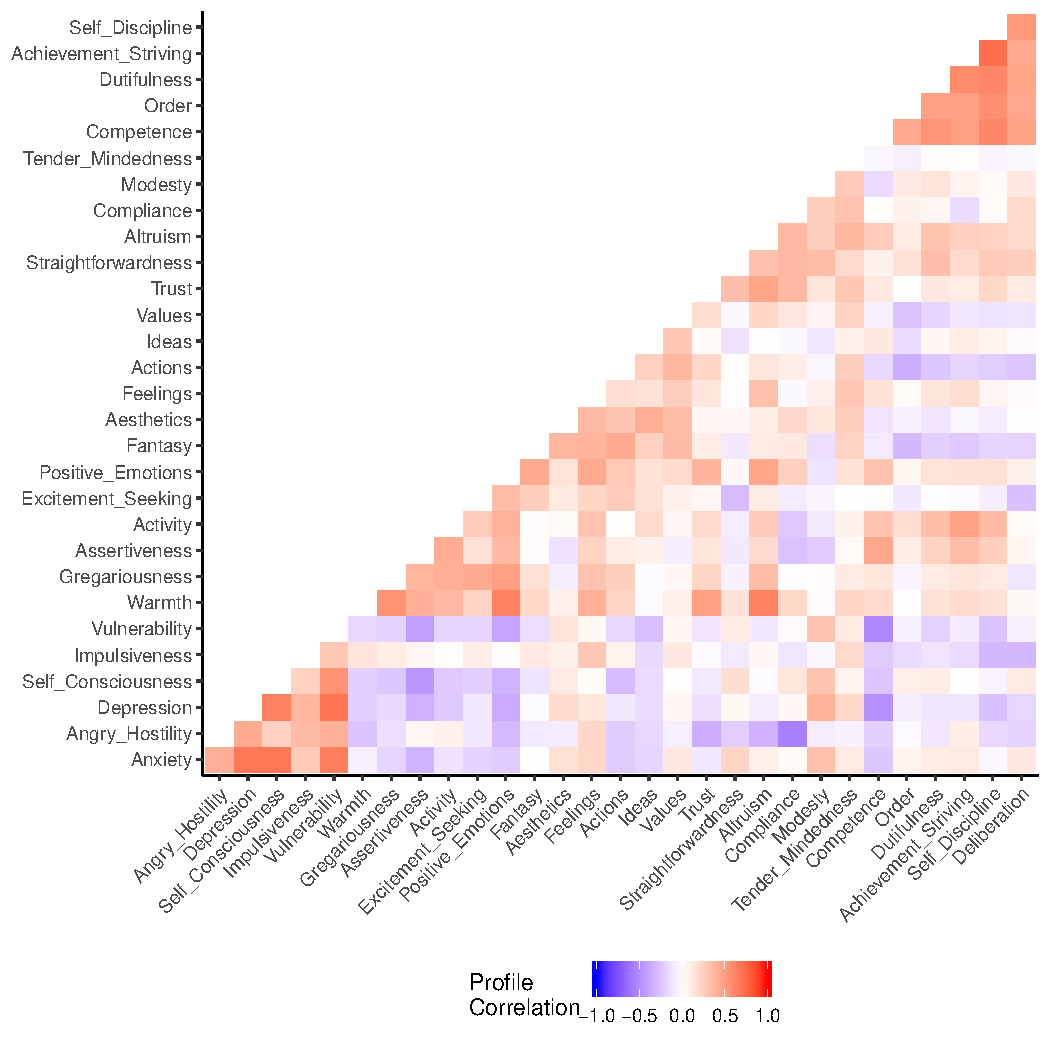
\includegraphics[width=\maxwidth]{figure/unnamed-chunk-6-1} 

\end{knitrout}

There appear to be intercorrelations among the variables.  

\subsubsection{KMO}
\begin{knitrout}
\definecolor{shadecolor}{rgb}{0.969, 0.969, 0.969}\color{fgcolor}\begin{kframe}
\begin{alltt}
\hlstd{(KMO1} \hlkwb{<-} \hlkwd{KMO}\hlstd{(r))}
\end{alltt}
\begin{verbatim}
## Kaiser-Meyer-Olkin factor adequacy
## Call: KMO(r = r)
## Overall MSA =  0.83
## MSA for each item = 
##              Anxiety      Angry_Hostility           Depression 
##                 0.83                 0.78                 0.82 
##   Self_Consciousness        Impulsiveness        Vulnerability 
##                 0.89                 0.83                 0.87 
##               Warmth       Gregariousness        Assertiveness 
##                 0.82                 0.84                 0.86 
##             Activity   Excitement_Seeking    Positive_Emotions 
##                 0.83                 0.79                 0.86 
##              Fantasy           Aesthetics             Feelings 
##                 0.79                 0.71                 0.82 
##              Actions                Ideas               Values 
##                 0.83                 0.68                 0.73 
##                Trust  Straightforwardness             Altruism 
##                 0.85                 0.72                 0.86 
##           Compliance              Modesty    Tender_Mindedness 
##                 0.73                 0.77                 0.78 
##           Competence                Order          Dutifulness 
##                 0.88                 0.86                 0.86 
## Achievement_Striving      Self_Discipline         Deliberation 
##                 0.85                 0.85                 0.84
\end{verbatim}
\end{kframe}
\end{knitrout}

The MSA for each item range from 0.68 to 0.89, with a mean of 0.81, indicating strong evidence for using a data reduction technique. 

\subsubsection{Bartlett's Test}
\begin{knitrout}
\definecolor{shadecolor}{rgb}{0.969, 0.969, 0.969}\color{fgcolor}\begin{kframe}
\begin{alltt}
\hlstd{(CB_1} \hlkwb{<-} \hlkwd{cortest.bartlett}\hlstd{(}\hlkwc{R}\hlstd{=r,}\hlkwc{n}\hlstd{=}\hlkwd{nrow}\hlstd{(dat2)))}
\end{alltt}
\begin{verbatim}
## $chisq
## [1] 3150.475
## 
## $p.value
## [1] 0
## 
## $df
## [1] 435
\end{verbatim}
\end{kframe}
\end{knitrout}

In addition, the $\chi^2$ value of the Bartlett test ($\chi^2$(435) = 3150.48), which indicates that the correlation matrix departs significantly from from an identity matrix (independence among indicators).  



\subsection{How Many Factors?}
Now that we have seen evidence suggesting that we should conduct a CFA or PCA, we need to determine how many factors we should extract. 
\subsubsection{Parallel Analysis (Scree Test)}
\begin{knitrout}
\definecolor{shadecolor}{rgb}{0.969, 0.969, 0.969}\color{fgcolor}\begin{kframe}
\begin{alltt}
\hlkwd{par}\hlstd{(}\hlkwc{mfrow}\hlstd{=}\hlkwd{c}\hlstd{(}\hlnum{1}\hlstd{,}\hlnum{2}\hlstd{))}
\hlstd{scree_1} \hlkwb{<-} \hlkwd{fa.parallel}\hlstd{(dat2} \hlopt \hlkwd{select}\hlstd{(}\hlopt{-}\hlstd{ID),} \hlkwc{fa}\hlstd{=}\hlstr{"both"}\hlstd{)}
\end{alltt}
\begin{verbatim}
## Parallel analysis suggests that the number of factors =  5  and the number of components =  5
\end{verbatim}
\begin{alltt}
\hlstd{scree_2} \hlkwb{<-} \hlkwd{fa.parallel}\hlstd{(r,} \hlkwc{fa} \hlstd{=} \hlstr{"both"}\hlstd{,} \hlkwc{n.obs} \hlstd{=} \hlkwd{nrow}\hlstd{(dat))}
\end{alltt}
\end{kframe}
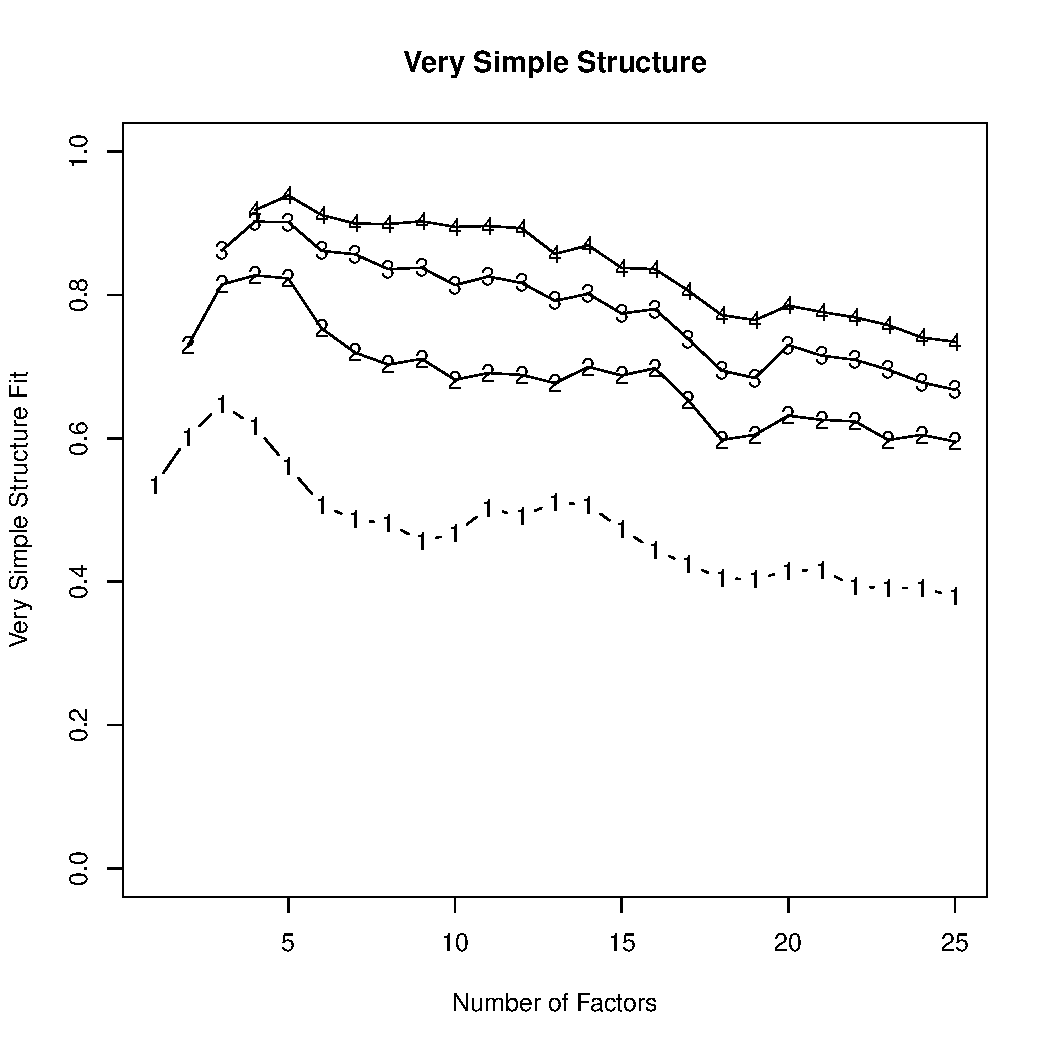
\includegraphics[width=\maxwidth]{figure/unnamed-chunk-9-1} 
\begin{kframe}\begin{verbatim}
## Parallel analysis suggests that the number of factors =  5  and the number of components =  5
\end{verbatim}
\end{kframe}
\end{knitrout}

Parallel analysis suggests 5 principal components and 5 factors. 

\subsubsection{VSS}
\begin{knitrout}
\definecolor{shadecolor}{rgb}{0.969, 0.969, 0.969}\color{fgcolor}\begin{kframe}
\begin{alltt}
\hlkwd{par}\hlstd{(}\hlkwc{mfrow} \hlstd{=} \hlkwd{c}\hlstd{(}\hlnum{1}\hlstd{,}\hlnum{1}\hlstd{))}
\hlstd{vss_1} \hlkwb{<-} \hlkwd{vss}\hlstd{(dat2} \hlopt \hlkwd{select}\hlstd{(}\hlopt{-}\hlstd{ID),} \hlkwc{n} \hlstd{=} \hlnum{25}\hlstd{,} \hlkwc{rotate} \hlstd{=} \hlstr{"none"}\hlstd{,} \hlkwc{fm} \hlstd{=} \hlstr{"pc"}\hlstd{)}
\end{alltt}
\end{kframe}
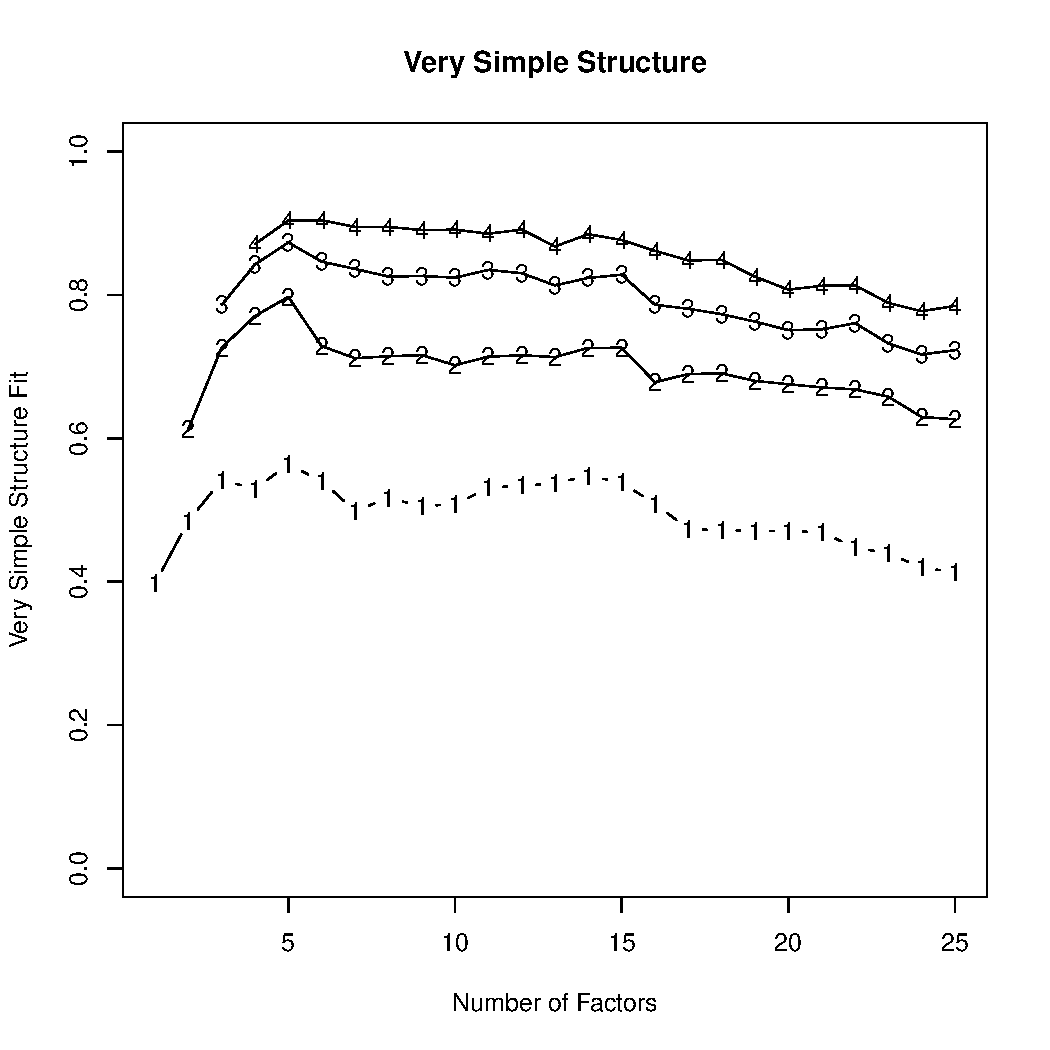
\includegraphics[width=\maxwidth]{figure/unnamed-chunk-10-1} 

\end{knitrout}

VSS also suggests 5 factors.  

\subsection{Exploratory Factor Analysis}
\begin{knitrout}
\definecolor{shadecolor}{rgb}{0.969, 0.969, 0.969}\color{fgcolor}\begin{kframe}
\begin{alltt}
\hlstd{fa_1} \hlkwb{<-} \hlkwd{fa}\hlstd{(dat2} \hlopt \hlkwd{select}\hlstd{(}\hlopt{-}\hlstd{ID),} \hlkwc{nfactors} \hlstd{=} \hlnum{5}\hlstd{,} \hlkwc{rotate} \hlstd{=} \hlstr{"none"}\hlstd{,} \hlkwc{scores} \hlstd{= T)}
\hlstd{fa_2} \hlkwb{<-} \hlkwd{fa}\hlstd{(dat2} \hlopt \hlkwd{select}\hlstd{(}\hlopt{-}\hlstd{ID),} \hlkwc{nfactors} \hlstd{=} \hlnum{5}\hlstd{,} \hlkwc{rotate} \hlstd{=} \hlstr{"varimax"}\hlstd{,} \hlkwc{scores} \hlstd{= T)}
\hlstd{fa_3} \hlkwb{<-} \hlkwd{fa}\hlstd{(dat2} \hlopt \hlkwd{select}\hlstd{(}\hlopt{-}\hlstd{ID),} \hlkwc{nfactors} \hlstd{=} \hlnum{5}\hlstd{,} \hlkwc{rotate} \hlstd{=} \hlstr{"oblimin"}\hlstd{,} \hlkwc{scores} \hlstd{= T)}

\hlstd{scores_1} \hlkwb{<-} \hlstd{fa_1}\hlopt{$}\hlstd{scores}
\hlstd{scores_2} \hlkwb{<-} \hlstd{fa_2}\hlopt{$}\hlstd{scores}
\hlstd{scores_3} \hlkwb{<-} \hlstd{fa_3}\hlopt{$}\hlstd{scores}

\hlcom{# unrotated}
\hlkwd{cor}\hlstd{(scores_1)} \hlopt \hlkwd{round}\hlstd{(.,} \hlnum{2}\hlstd{)}
\end{alltt}
\begin{verbatim}
##       MR1   MR2   MR3   MR4   MR5
## MR1  1.00  0.00 -0.01 -0.01  0.00
## MR2  0.00  1.00 -0.01 -0.01 -0.02
## MR3 -0.01 -0.01  1.00  0.01 -0.01
## MR4 -0.01 -0.01  0.01  1.00  0.00
## MR5  0.00 -0.02 -0.01  0.00  1.00
\end{verbatim}
\begin{alltt}
\hlcom{# varimax rotation}
\hlkwd{cor}\hlstd{(scores_2)} \hlopt \hlkwd{round}\hlstd{(.,} \hlnum{2}\hlstd{)}
\end{alltt}
\begin{verbatim}
##       MR2   MR3   MR1  MR4   MR5
## MR2  1.00 -0.01  0.03 0.02 -0.03
## MR3 -0.01  1.00 -0.02 0.00  0.01
## MR1  0.03 -0.02  1.00 0.02  0.06
## MR4  0.02  0.00  0.02 1.00  0.03
## MR5 -0.03  0.01  0.06 0.03  1.00
\end{verbatim}
\begin{alltt}
\hlcom{# oblimin rotation}
\hlkwd{cor}\hlstd{(scores_3)} \hlopt \hlkwd{round}\hlstd{(.,} \hlnum{2}\hlstd{)}
\end{alltt}
\begin{verbatim}
##       MR2   MR3   MR1   MR4   MR5
## MR2  1.00 -0.11  0.19  0.06 -0.08
## MR3 -0.11  1.00 -0.16 -0.01 -0.05
## MR1  0.19 -0.16  1.00  0.06  0.32
## MR4  0.06 -0.01  0.06  1.00  0.07
## MR5 -0.08 -0.05  0.32  0.07  1.00
\end{verbatim}
\end{kframe}
\end{knitrout}


The two models fit the data relatively well ($RMSEA_{unrotated} = 0.07$, $RMSEA_{varimax} = 0.07$, $RMSEA_{oblimin} = 0.07$, $TLI_{unrotated} = 0.87$; $TLI_{varimax} = 0.87$; $TLI_{oblimin} = 0.87$).  

We can also look at the communalities: 

\begin{knitrout}
\definecolor{shadecolor}{rgb}{0.969, 0.969, 0.969}\color{fgcolor}\begin{kframe}
\begin{alltt}
\hlkwd{tibble}\hlstd{(}\hlkwc{Facet} \hlstd{=} \hlkwd{names}\hlstd{(fa_1}\hlopt{$}\hlstd{communalities),}
       \hlkwc{Unrotated} \hlstd{= fa_1}\hlopt{$}\hlstd{communalities,}
       \hlkwc{Varimax} \hlstd{= fa_2}\hlopt{$}\hlstd{communalities,}
       \hlkwc{Oblimin} \hlstd{= fa_3}\hlopt{$}\hlstd{communalities)} \hlopt
  \hlkwd{mutate}\hlstd{(}\hlkwc{Facet} \hlstd{=} \hlkwd{str_replace_all}\hlstd{(Facet,} \hlstr{"_"}\hlstd{,} \hlstr{" "}\hlstd{))} \hlopt
  \hlkwd{kable}\hlstd{(.,} \hlstr{"latex"}\hlstd{,} \hlkwc{booktabs} \hlstd{= T,} \hlkwc{escape} \hlstd{= F,} \hlkwc{digits} \hlstd{=} \hlnum{2}\hlstd{,}
        \hlkwc{caption} \hlstd{=} \hlstr{"Communalities"}\hlstd{)} \hlopt
  \hlkwd{kable_styling}\hlstd{(}\hlkwc{full_width} \hlstd{= F)}
\end{alltt}
\end{kframe}\begin{table}

\caption{\label{tab:unnamed-chunk-12}Communalities}
\centering
\begin{tabular}[t]{lrrr}
\toprule
Facet & Unrotated & Varimax & Oblimin\\
\midrule
Anxiety & 0.73 & 0.73 & 0.73\\
Angry Hostility & 0.72 & 0.72 & 0.72\\
Depression & 0.75 & 0.75 & 0.75\\
Self Consciousness & 0.60 & 0.60 & 0.60\\
Impulsiveness & 0.36 & 0.36 & 0.36\\
\addlinespace
Vulnerability & 0.68 & 0.68 & 0.68\\
Warmth & 0.72 & 0.72 & 0.72\\
Gregariousness & 0.50 & 0.50 & 0.50\\
Assertiveness & 0.52 & 0.52 & 0.52\\
Activity & 0.48 & 0.48 & 0.48\\
\addlinespace
Excitement Seeking & 0.26 & 0.26 & 0.26\\
Positive Emotions & 0.65 & 0.65 & 0.65\\
Fantasy & 0.47 & 0.47 & 0.47\\
Aesthetics & 0.54 & 0.54 & 0.54\\
Feelings & 0.57 & 0.57 & 0.57\\
\addlinespace
Actions & 0.44 & 0.44 & 0.44\\
Ideas & 0.46 & 0.46 & 0.46\\
Values & 0.33 & 0.33 & 0.33\\
Trust & 0.41 & 0.41 & 0.41\\
Straightforwardness & 0.39 & 0.39 & 0.39\\
\addlinespace
Altruism & 0.64 & 0.64 & 0.64\\
Compliance & 0.63 & 0.63 & 0.63\\
Modesty & 0.32 & 0.32 & 0.32\\
Tender Mindedness & 0.29 & 0.29 & 0.29\\
Competence & 0.64 & 0.64 & 0.64\\
\addlinespace
Order & 0.46 & 0.46 & 0.46\\
Dutifulness & 0.58 & 0.58 & 0.58\\
Achievement Striving & 0.70 & 0.70 & 0.70\\
Self Discipline & 0.72 & 0.72 & 0.72\\
Deliberation & 0.51 & 0.51 & 0.51\\
\bottomrule
\end{tabular}
\end{table}


\end{knitrout}

THe communalities are identical across models but suggest that the latent factors explain a considerable amount of the variance in most variables.  

How much variance is explained?
\begin{knitrout}
\definecolor{shadecolor}{rgb}{0.969, 0.969, 0.969}\color{fgcolor}\begin{kframe}
\begin{alltt}
\hlstd{fa_1}\hlopt{$}\hlstd{Vaccounted} \hlopt \hlstd{data.frame} \hlopt \hlkwd{mutate}\hlstd{(}\hlkwc{Measure} \hlstd{=} \hlkwd{rownames}\hlstd{(.),} \hlkwc{Rotate} \hlstd{=} \hlstr{"Unrotated"}\hlstd{)} \hlopt
  \hlkwd{full_join}\hlstd{(}
    \hlstd{fa_1}\hlopt{$}\hlstd{Vaccounted} \hlopt \hlstd{data.frame} \hlopt \hlkwd{mutate}\hlstd{(}\hlkwc{Measure} \hlstd{=} \hlkwd{rownames}\hlstd{(.),} \hlkwc{Rotate} \hlstd{=} \hlstr{"Varimax"}\hlstd{)}
  \hlstd{)} \hlopt
  \hlkwd{full_join}\hlstd{(}
    \hlstd{fa_1}\hlopt{$}\hlstd{Vaccounted} \hlopt \hlstd{data.frame} \hlopt \hlkwd{mutate}\hlstd{(}\hlkwc{Measure} \hlstd{=} \hlkwd{rownames}\hlstd{(.),} \hlkwc{Rotate} \hlstd{=} \hlstr{"Oblimin"}\hlstd{)}
  \hlstd{)} \hlopt
  \hlkwd{select}\hlstd{(Measure,} \hlkwd{everything}\hlstd{(),} \hlopt{-}\hlstd{Rotate)} \hlopt
  \hlkwd{kable}\hlstd{(.,} \hlstr{"latex"}\hlstd{,} \hlkwc{escape} \hlstd{= F,} \hlkwc{booktabs} \hlstd{= T,} \hlkwc{digits} \hlstd{=} \hlnum{2}\hlstd{,}
        \hlkwc{caption} \hlstd{=} \hlstr{"Variance Explained"}\hlstd{)} \hlopt
  \hlkwd{group_rows}\hlstd{(}\hlstr{"Unrotated"}\hlstd{,} \hlnum{1}\hlstd{,}\hlnum{5}\hlstd{)} \hlopt
  \hlkwd{group_rows}\hlstd{(}\hlstr{"Varimax"}\hlstd{,} \hlnum{6}\hlstd{,} \hlnum{10}\hlstd{)} \hlopt
  \hlkwd{group_rows}\hlstd{(}\hlstr{"Oblimin"}\hlstd{,} \hlnum{11}\hlstd{,} \hlnum{15}\hlstd{)}
\end{alltt}
\end{kframe}\begin{table}

\caption{\label{tab:unnamed-chunk-13}Variance Explained}
\centering
\begin{tabular}[t]{lrrrrr}
\toprule
Measure & MR1 & MR2 & MR3 & MR4 & MR5\\
\midrule
\addlinespace[0.3em]
\multicolumn{6}{l}{\textbf{Unrotated}}\\
\hspace{1em}SS loadings & 5.36 & 3.75 & 3.35 & 2.23 & \vphantom{2} 1.36\\
\hspace{1em}Proportion Var & 0.18 & 0.13 & 0.11 & 0.07 & \vphantom{2} 0.05\\
\hspace{1em}Cumulative Var & 0.18 & 0.30 & 0.42 & 0.49 & \vphantom{2} 0.54\\
\hspace{1em}Proportion Explained & 0.33 & 0.23 & 0.21 & 0.14 & \vphantom{2} 0.08\\
\hspace{1em}Cumulative Proportion & 0.33 & 0.57 & 0.78 & 0.92 & \vphantom{2} 1.00\\
\addlinespace[0.3em]
\multicolumn{6}{l}{\textbf{Varimax}}\\
\hspace{1em}SS loadings & 5.36 & 3.75 & 3.35 & 2.23 & \vphantom{1} 1.36\\
\hspace{1em}Proportion Var & 0.18 & 0.13 & 0.11 & 0.07 & \vphantom{1} 0.05\\
\hspace{1em}Cumulative Var & 0.18 & 0.30 & 0.42 & 0.49 & \vphantom{1} 0.54\\
\hspace{1em}Proportion Explained & 0.33 & 0.23 & 0.21 & 0.14 & \vphantom{1} 0.08\\
\hspace{1em}Cumulative Proportion & 0.33 & 0.57 & 0.78 & 0.92 & \vphantom{1} 1.00\\
\addlinespace[0.3em]
\multicolumn{6}{l}{\textbf{Oblimin}}\\
\hspace{1em}SS loadings & 5.36 & 3.75 & 3.35 & 2.23 & 1.36\\
\hspace{1em}Proportion Var & 0.18 & 0.13 & 0.11 & 0.07 & 0.05\\
\hspace{1em}Cumulative Var & 0.18 & 0.30 & 0.42 & 0.49 & 0.54\\
\hspace{1em}Proportion Explained & 0.33 & 0.23 & 0.21 & 0.14 & 0.08\\
\hspace{1em}Cumulative Proportion & 0.33 & 0.57 & 0.78 & 0.92 & 1.00\\
\bottomrule
\end{tabular}
\end{table}


\end{knitrout}


But we aren't just concerned with model fit. We are also generally interested in naming the factors. 

There's no way for me to pretend I don't have expectations for how the data should come out. So let's look at the rotated and unrotated solutions and see if we managed to recover the Big 5. 
\begin{kframe}
\begin{alltt}
\hlstd{fa_1}\hlopt{$}\hlstd{Structure} \hlopt \hlstd{unclass} \hlopt
  \hlstd{data.frame} \hlopt
  \hlkwd{mutate}\hlstd{(}\hlkwc{Facet} \hlstd{=} \hlkwd{rownames}\hlstd{(.))} \hlopt
  \hlkwd{full_join}\hlstd{(source)} \hlopt
  \hlkwd{select}\hlstd{(Factor, Facet, MR1, MR2, MR3, MR4, MR5)} \hlopt
  \hlkwd{mutate_at}\hlstd{(}\hlkwd{vars}\hlstd{(MR1}\hlopt{:}\hlstd{MR5),} \hlkwd{funs}\hlstd{(}\hlkwd{round}\hlstd{(.,} \hlnum{2}\hlstd{)))} \hlopt
  \hlkwd{mutate_at}\hlstd{(}\hlkwd{vars}\hlstd{(MR1}\hlopt{:}\hlstd{MR5),} \hlkwd{funs}\hlstd{(}\hlkwd{cell_spec}\hlstd{(.,} \hlstr{"latex"}\hlstd{,}
        \hlkwc{background} \hlstd{=} \hlkwd{ifelse}\hlstd{((.)} \hlopt{>} \hlnum{.5}\hlstd{,} \hlstr{"yellow"}\hlstd{,} \hlstr{"white"}\hlstd{))))} \hlopt
  \hlkwd{mutate}\hlstd{(}\hlkwc{Facet} \hlstd{=} \hlkwd{str_replace_all}\hlstd{(Facet,} \hlstr{"_"}\hlstd{,} \hlstr{" "}\hlstd{))} \hlopt
  \hlkwd{kable}\hlstd{(.,} \hlstr{"latex"}\hlstd{,} \hlkwc{escape} \hlstd{= F,} \hlkwc{booktabs} \hlstd{= T,}
        \hlkwc{caption} \hlstd{=} \hlstr{"Unrotated Solution"}\hlstd{)} \hlopt
  \hlkwd{kable_styling}\hlstd{(}\hlkwc{full_width} \hlstd{= F)}
\end{alltt}
\end{kframe}\begin{table}

\caption{\label{tab:unnamed-chunk-14}Unrotated Solution}
\centering
\begin{tabular}[t]{lllllll}
\toprule
Factor & Facet & MR1 & MR2 & MR3 & MR4 & MR5\\
\midrule
Neuroticism & Anxiety & \cellcolor{white}{-0.44} & \cellcolor{white}{-0.25} & \cellcolor{yellow}{0.66} & \cellcolor{white}{0.21} & \cellcolor{white}{0.06}\\
Neuroticism & Angry Hostility & \cellcolor{white}{-0.44} & \cellcolor{white}{-0.13} & \cellcolor{white}{0.04} & \cellcolor{yellow}{0.71} & \cellcolor{white}{0.02}\\
Neuroticism & Depression & \cellcolor{white}{-0.63} & \cellcolor{white}{-0.04} & \cellcolor{yellow}{0.56} & \cellcolor{white}{0.21} & \cellcolor{white}{-0.01}\\
Neuroticism & Self Consciousness & \cellcolor{white}{-0.49} & \cellcolor{white}{-0.3} & \cellcolor{yellow}{0.52} & \cellcolor{white}{0.02} & \cellcolor{white}{0.05}\\
Neuroticism & Impulsiveness & \cellcolor{white}{-0.23} & \cellcolor{white}{0.25} & \cellcolor{white}{0.28} & \cellcolor{white}{0.37} & \cellcolor{white}{-0.18}\\
\addlinespace
Neuroticism & Vulnerability & \cellcolor{white}{-0.63} & \cellcolor{white}{-0.12} & \cellcolor{white}{0.48} & \cellcolor{white}{0.14} & \cellcolor{white}{-0.1}\\
Extraversion & Warmth & \cellcolor{yellow}{0.61} & \cellcolor{white}{0.28} & \cellcolor{white}{0.36} & \cellcolor{white}{0.09} & \cellcolor{white}{-0.36}\\
Extraversion & Gregariousness & \cellcolor{white}{0.48} & \cellcolor{white}{0.29} & \cellcolor{white}{0.12} & \cellcolor{white}{0.26} & \cellcolor{white}{-0.32}\\
Extraversion & Assertiveness & \cellcolor{yellow}{0.58} & \cellcolor{white}{0.04} & \cellcolor{white}{-0.16} & \cellcolor{white}{0.38} & \cellcolor{white}{-0.12}\\
Extraversion & Activity & \cellcolor{yellow}{0.54} & \cellcolor{white}{-0.01} & \cellcolor{white}{0.07} & \cellcolor{white}{0.44} & \cellcolor{white}{0.02}\\
\addlinespace
Extraversion & Excitement Seeking & \cellcolor{white}{0.24} & \cellcolor{white}{0.38} & \cellcolor{white}{-0.03} & \cellcolor{white}{0.23} & \cellcolor{white}{-0.02}\\
Extraversion & Positive Emotions & \cellcolor{yellow}{0.69} & \cellcolor{white}{0.36} & \cellcolor{white}{0.19} & \cellcolor{white}{0.05} & \cellcolor{white}{-0.04}\\
Openness & Fantasy & \cellcolor{white}{0.13} & \cellcolor{yellow}{0.59} & \cellcolor{white}{0.17} & \cellcolor{white}{0.02} & \cellcolor{white}{0.27}\\
Openness & Aesthetics & \cellcolor{white}{0} & \cellcolor{white}{0.32} & \cellcolor{white}{0.38} & \cellcolor{white}{-0.05} & \cellcolor{yellow}{0.54}\\
Openness & Feelings & \cellcolor{white}{0.29} & \cellcolor{white}{0.26} & \cellcolor{white}{0.47} & \cellcolor{white}{0.41} & \cellcolor{white}{0.17}\\
\addlinespace
Openness & Actions & \cellcolor{white}{0.17} & \cellcolor{yellow}{0.62} & \cellcolor{white}{0.07} & \cellcolor{white}{-0.1} & \cellcolor{white}{0.12}\\
Openness & Ideas & \cellcolor{white}{0.22} & \cellcolor{white}{0.24} & \cellcolor{white}{-0.04} & \cellcolor{white}{-0.01} & \cellcolor{yellow}{0.59}\\
Openness & Values & \cellcolor{white}{0.04} & \cellcolor{white}{0.4} & \cellcolor{white}{0.27} & \cellcolor{white}{-0.04} & \cellcolor{white}{0.3}\\
Agreeableness & Trust & \cellcolor{white}{0.42} & \cellcolor{white}{0.14} & \cellcolor{white}{0.33} & \cellcolor{white}{-0.26} & \cellcolor{white}{-0.19}\\
Agreeableness & Straightforwardness & \cellcolor{white}{0.13} & \cellcolor{white}{-0.26} & \cellcolor{white}{0.42} & \cellcolor{white}{-0.35} & \cellcolor{white}{-0.1}\\
\addlinespace
Agreeableness & Altruism & \cellcolor{yellow}{0.53} & \cellcolor{white}{0.07} & \cellcolor{yellow}{0.54} & \cellcolor{white}{-0.12} & \cellcolor{white}{-0.22}\\
Agreeableness & Compliance & \cellcolor{white}{0.13} & \cellcolor{white}{0.07} & \cellcolor{white}{0.41} & \cellcolor{white}{-0.66} & \cellcolor{white}{-0.07}\\
Agreeableness & Modesty & \cellcolor{white}{-0.12} & \cellcolor{white}{-0.15} & \cellcolor{white}{0.49} & \cellcolor{white}{-0.18} & \cellcolor{white}{-0.07}\\
Agreeableness & Tender Mindedness & \cellcolor{white}{0.1} & \cellcolor{white}{0.23} & \cellcolor{white}{0.47} & \cellcolor{white}{-0.08} & \cellcolor{white}{0.02}\\
Conscientiousness & Competence & \cellcolor{yellow}{0.68} & \cellcolor{white}{-0.38} & \cellcolor{white}{-0.11} & \cellcolor{white}{0.05} & \cellcolor{white}{0.15}\\
\addlinespace
Conscientiousness & Order & \cellcolor{white}{0.28} & \cellcolor{white}{-0.61} & \cellcolor{white}{0.09} & \cellcolor{white}{0.04} & \cellcolor{white}{0.05}\\
Conscientiousness & Dutifulness & \cellcolor{white}{0.47} & \cellcolor{white}{-0.55} & \cellcolor{white}{0.22} & \cellcolor{white}{0.08} & \cellcolor{white}{0.05}\\
Conscientiousness & Achievement Striving & \cellcolor{white}{0.49} & \cellcolor{white}{-0.55} & \cellcolor{white}{0.18} & \cellcolor{white}{0.31} & \cellcolor{white}{0.16}\\
Conscientiousness & Self Discipline & \cellcolor{yellow}{0.58} & \cellcolor{white}{-0.59} & \cellcolor{white}{0.09} & \cellcolor{white}{0.02} & \cellcolor{white}{0.16}\\
Conscientiousness & Deliberation & \cellcolor{white}{0.31} & \cellcolor{white}{-0.55} & \cellcolor{white}{0.16} & \cellcolor{white}{-0.2} & \cellcolor{white}{0.2}\\
\bottomrule
\end{tabular}
\end{table}



\begin{kframe}
\begin{alltt}
\hlstd{fa_2}\hlopt{$}\hlstd{Structure} \hlopt \hlstd{unclass} \hlopt
  \hlstd{data.frame} \hlopt
  \hlkwd{mutate}\hlstd{(}\hlkwc{Facet} \hlstd{=} \hlkwd{rownames}\hlstd{(.))} \hlopt
  \hlkwd{full_join}\hlstd{(source)} \hlopt
  \hlkwd{select}\hlstd{(Factor, Facet, MR1, MR2, MR3, MR4, MR5)} \hlopt
  \hlkwd{mutate_at}\hlstd{(}\hlkwd{vars}\hlstd{(MR1}\hlopt{:}\hlstd{MR5),} \hlkwd{funs}\hlstd{(}\hlkwd{round}\hlstd{(.,} \hlnum{2}\hlstd{)))} \hlopt
  \hlkwd{mutate_at}\hlstd{(}\hlkwd{vars}\hlstd{(MR1}\hlopt{:}\hlstd{MR5),} \hlkwd{funs}\hlstd{(}\hlkwd{cell_spec}\hlstd{(.,} \hlstr{"latex"}\hlstd{,}
        \hlkwc{background} \hlstd{=} \hlkwd{ifelse}\hlstd{(}\hlkwd{abs}\hlstd{(.)} \hlopt{>} \hlnum{.5}\hlstd{,} \hlstr{"yellow"}\hlstd{,} \hlstr{"white"}\hlstd{))))} \hlopt
  \hlkwd{mutate}\hlstd{(}\hlkwc{Facet} \hlstd{=} \hlkwd{str_replace_all}\hlstd{(Facet,} \hlstr{"_"}\hlstd{,} \hlstr{" "}\hlstd{))} \hlopt
  \hlkwd{kable}\hlstd{(.,} \hlstr{"latex"}\hlstd{,} \hlkwc{escape} \hlstd{= F,} \hlkwc{booktabs} \hlstd{= T,}
        \hlkwc{caption} \hlstd{=} \hlstr{"Varimax Rotated Solution"}\hlstd{)} \hlopt
  \hlkwd{kable_styling}\hlstd{(}\hlkwc{full_width} \hlstd{= F)}
\end{alltt}
\end{kframe}\begin{table}

\caption{\label{tab:unnamed-chunk-15}Varimax Rotated Solution}
\centering
\begin{tabular}[t]{lllllll}
\toprule
Factor & Facet & MR1 & MR2 & MR3 & MR4 & MR5\\
\midrule
Neuroticism & Anxiety & \cellcolor{white}{-0.09} & \cellcolor{white}{0.12} & \cellcolor{yellow}{0.84} & \cellcolor{white}{0.04} & \cellcolor{white}{0.06}\\
Neuroticism & Angry Hostility & \cellcolor{white}{0.05} & \cellcolor{white}{-0.02} & \cellcolor{yellow}{0.53} & \cellcolor{yellow}{-0.66} & \cellcolor{white}{-0.1}\\
Neuroticism & Depression & \cellcolor{white}{-0.13} & \cellcolor{white}{-0.18} & \cellcolor{yellow}{0.84} & \cellcolor{white}{-0.03} & \cellcolor{white}{0.04}\\
Neuroticism & Self Consciousness & \cellcolor{white}{-0.27} & \cellcolor{white}{0.07} & \cellcolor{yellow}{0.71} & \cellcolor{white}{0.11} & \cellcolor{white}{-0.02}\\
Neuroticism & Impulsiveness & \cellcolor{white}{0.3} & \cellcolor{white}{-0.27} & \cellcolor{white}{0.42} & \cellcolor{white}{-0.15} & \cellcolor{white}{0.02}\\
\addlinespace
Neuroticism & Vulnerability & \cellcolor{white}{-0.18} & \cellcolor{white}{-0.17} & \cellcolor{yellow}{0.78} & \cellcolor{white}{0.01} & \cellcolor{white}{-0.08}\\
Extraversion & Warmth & \cellcolor{yellow}{0.76} & \cellcolor{white}{0.06} & \cellcolor{white}{-0.06} & \cellcolor{white}{0.36} & \cellcolor{white}{0.03}\\
Extraversion & Gregariousness & \cellcolor{yellow}{0.69} & \cellcolor{white}{-0.02} & \cellcolor{white}{-0.13} & \cellcolor{white}{0.07} & \cellcolor{white}{-0.02}\\
Extraversion & Assertiveness & \cellcolor{yellow}{0.55} & \cellcolor{white}{0.26} & \cellcolor{white}{-0.32} & \cellcolor{white}{-0.21} & \cellcolor{white}{-0.05}\\
Extraversion & Activity & \cellcolor{yellow}{0.55} & \cellcolor{white}{0.36} & \cellcolor{white}{-0.1} & \cellcolor{white}{-0.19} & \cellcolor{white}{0.1}\\
\addlinespace
Extraversion & Excitement Seeking & \cellcolor{white}{0.4} & \cellcolor{white}{-0.15} & \cellcolor{white}{-0.15} & \cellcolor{white}{-0.11} & \cellcolor{white}{0.19}\\
Extraversion & Positive Emotions & \cellcolor{yellow}{0.64} & \cellcolor{white}{0.11} & \cellcolor{white}{-0.29} & \cellcolor{white}{0.24} & \cellcolor{white}{0.29}\\
Openness & Fantasy & \cellcolor{white}{0.25} & \cellcolor{white}{-0.27} & \cellcolor{white}{-0.07} & \cellcolor{white}{0.05} & \cellcolor{yellow}{0.57}\\
Openness & Aesthetics & \cellcolor{white}{-0.02} & \cellcolor{white}{-0.02} & \cellcolor{white}{0.18} & \cellcolor{white}{0.11} & \cellcolor{yellow}{0.7}\\
Openness & Feelings & \cellcolor{yellow}{0.54} & \cellcolor{white}{0.14} & \cellcolor{white}{0.27} & \cellcolor{white}{-0.05} & \cellcolor{white}{0.43}\\
\addlinespace
Openness & Actions & \cellcolor{white}{0.25} & \cellcolor{white}{-0.35} & \cellcolor{white}{-0.19} & \cellcolor{white}{0.15} & \cellcolor{white}{0.44}\\
Openness & Ideas & \cellcolor{white}{-0.04} & \cellcolor{white}{0.11} & \cellcolor{white}{-0.24} & \cellcolor{white}{-0.1} & \cellcolor{yellow}{0.61}\\
Openness & Values & \cellcolor{white}{0.11} & \cellcolor{white}{-0.15} & \cellcolor{white}{0.07} & \cellcolor{white}{0.12} & \cellcolor{yellow}{0.52}\\
Agreeableness & Trust & \cellcolor{white}{0.33} & \cellcolor{white}{0.07} & \cellcolor{white}{-0.08} & \cellcolor{yellow}{0.53} & \cellcolor{white}{0.07}\\
Agreeableness & Straightforwardness & \cellcolor{white}{-0.04} & \cellcolor{white}{0.26} & \cellcolor{white}{0.18} & \cellcolor{yellow}{0.54} & \cellcolor{white}{-0.06}\\
\addlinespace
Agreeableness & Altruism & \cellcolor{yellow}{0.51} & \cellcolor{white}{0.23} & \cellcolor{white}{0.07} & \cellcolor{yellow}{0.56} & \cellcolor{white}{0.09}\\
Agreeableness & Compliance & \cellcolor{white}{-0.09} & \cellcolor{white}{-0.03} & \cellcolor{white}{0.01} & \cellcolor{yellow}{0.78} & \cellcolor{white}{0.13}\\
Agreeableness & Modesty & \cellcolor{white}{-0.05} & \cellcolor{white}{0.09} & \cellcolor{white}{0.41} & \cellcolor{white}{0.38} & \cellcolor{white}{0}\\
Agreeableness & Tender Mindedness & \cellcolor{white}{0.23} & \cellcolor{white}{-0.05} & \cellcolor{white}{0.23} & \cellcolor{white}{0.33} & \cellcolor{white}{0.28}\\
Conscientiousness & Competence & \cellcolor{white}{0.19} & \cellcolor{yellow}{0.68} & \cellcolor{white}{-0.38} & \cellcolor{white}{0.02} & \cellcolor{white}{0}\\
\addlinespace
Conscientiousness & Order & \cellcolor{white}{-0.04} & \cellcolor{yellow}{0.65} & \cellcolor{white}{0.04} & \cellcolor{white}{0.05} & \cellcolor{white}{-0.19}\\
Conscientiousness & Dutifulness & \cellcolor{white}{0.15} & \cellcolor{yellow}{0.73} & \cellcolor{white}{0.03} & \cellcolor{white}{0.13} & \cellcolor{white}{-0.1}\\
Conscientiousness & Achievement Striving & \cellcolor{white}{0.22} & \cellcolor{yellow}{0.8} & \cellcolor{white}{0.05} & \cellcolor{white}{-0.09} & \cellcolor{white}{-0.01}\\
Conscientiousness & Self Discipline & \cellcolor{white}{0.08} & \cellcolor{yellow}{0.82} & \cellcolor{white}{-0.15} & \cellcolor{white}{0.11} & \cellcolor{white}{-0.05}\\
Conscientiousness & Deliberation & \cellcolor{white}{-0.17} & \cellcolor{yellow}{0.65} & \cellcolor{white}{-0.03} & \cellcolor{white}{0.25} & \cellcolor{white}{-0.02}\\
\bottomrule
\end{tabular}
\end{table}



\begin{kframe}
\begin{alltt}
\hlstd{fa_3}\hlopt{$}\hlstd{Structure} \hlopt \hlstd{unclass} \hlopt
  \hlstd{data.frame} \hlopt
  \hlkwd{mutate}\hlstd{(}\hlkwc{Facet} \hlstd{=} \hlkwd{rownames}\hlstd{(.))} \hlopt
  \hlkwd{full_join}\hlstd{(source)} \hlopt
  \hlkwd{select}\hlstd{(Factor, Facet, MR1, MR2, MR3, MR4, MR5)} \hlopt
  \hlkwd{mutate_at}\hlstd{(}\hlkwd{vars}\hlstd{(MR1}\hlopt{:}\hlstd{MR5),} \hlkwd{funs}\hlstd{(}\hlkwd{round}\hlstd{(.,} \hlnum{2}\hlstd{)))} \hlopt
  \hlkwd{mutate_at}\hlstd{(}\hlkwd{vars}\hlstd{(MR1}\hlopt{:}\hlstd{MR5),} \hlkwd{funs}\hlstd{(}\hlkwd{cell_spec}\hlstd{(.,} \hlstr{"latex"}\hlstd{,}
        \hlkwc{background} \hlstd{=} \hlkwd{ifelse}\hlstd{(}\hlkwd{abs}\hlstd{(.)} \hlopt{>} \hlnum{.5}\hlstd{,} \hlstr{"yellow"}\hlstd{,} \hlstr{"white"}\hlstd{))))} \hlopt
  \hlkwd{mutate}\hlstd{(}\hlkwc{Facet} \hlstd{=} \hlkwd{str_replace_all}\hlstd{(Facet,} \hlstr{"_"}\hlstd{,} \hlstr{" "}\hlstd{))} \hlopt
  \hlkwd{kable}\hlstd{(.,} \hlstr{"latex"}\hlstd{,} \hlkwc{escape} \hlstd{= F,} \hlkwc{booktabs} \hlstd{= T,}
        \hlkwc{caption} \hlstd{=} \hlstr{"Oblimin Rotated Solution"}\hlstd{)} \hlopt
  \hlkwd{kable_styling}\hlstd{(}\hlkwc{full_width} \hlstd{= F)}
\end{alltt}
\end{kframe}\begin{table}

\caption{\label{tab:unnamed-chunk-16}Oblimin Rotated Solution}
\centering
\begin{tabular}[t]{lllllll}
\toprule
Factor & Facet & MR1 & MR2 & MR3 & MR4 & MR5\\
\midrule
Neuroticism & Anxiety & \cellcolor{white}{-0.08} & \cellcolor{white}{0.06} & \cellcolor{yellow}{0.84} & \cellcolor{white}{-0.02} & \cellcolor{white}{0.02}\\
Neuroticism & Angry Hostility & \cellcolor{white}{-0.16} & \cellcolor{white}{-0.09} & \cellcolor{white}{0.47} & \cellcolor{yellow}{-0.71} & \cellcolor{white}{-0.13}\\
Neuroticism & Depression & \cellcolor{white}{-0.15} & \cellcolor{white}{-0.25} & \cellcolor{yellow}{0.85} & \cellcolor{white}{-0.08} & \cellcolor{white}{0}\\
Neuroticism & Self Consciousness & \cellcolor{white}{-0.24} & \cellcolor{white}{0.01} & \cellcolor{yellow}{0.74} & \cellcolor{white}{0.1} & \cellcolor{white}{-0.09}\\
Neuroticism & Impulsiveness & \cellcolor{white}{0.22} & \cellcolor{white}{-0.27} & \cellcolor{white}{0.37} & \cellcolor{white}{-0.26} & \cellcolor{white}{0.06}\\
\addlinespace
Neuroticism & Vulnerability & \cellcolor{white}{-0.2} & \cellcolor{white}{-0.23} & \cellcolor{yellow}{0.8} & \cellcolor{white}{-0.03} & \cellcolor{white}{-0.13}\\
Extraversion & Warmth & \cellcolor{yellow}{0.84} & \cellcolor{white}{0.16} & \cellcolor{white}{-0.15} & \cellcolor{white}{0.17} & \cellcolor{white}{0.17}\\
Extraversion & Gregariousness & \cellcolor{yellow}{0.68} & \cellcolor{white}{0.06} & \cellcolor{white}{-0.22} & \cellcolor{white}{-0.1} & \cellcolor{white}{0.1}\\
Extraversion & Assertiveness & \cellcolor{white}{0.48} & \cellcolor{white}{0.31} & \cellcolor{white}{-0.41} & \cellcolor{white}{-0.31} & \cellcolor{white}{0.04}\\
Extraversion & Activity & \cellcolor{white}{0.5} & \cellcolor{white}{0.4} & \cellcolor{white}{-0.2} & \cellcolor{white}{-0.3} & \cellcolor{white}{0.18}\\
\addlinespace
Extraversion & Excitement Seeking & \cellcolor{white}{0.36} & \cellcolor{white}{-0.12} & \cellcolor{white}{-0.21} & \cellcolor{white}{-0.19} & \cellcolor{white}{0.26}\\
Extraversion & Positive Emotions & \cellcolor{yellow}{0.72} & \cellcolor{white}{0.18} & \cellcolor{white}{-0.36} & \cellcolor{white}{0.12} & \cellcolor{white}{0.41}\\
Openness & Fantasy & \cellcolor{white}{0.28} & \cellcolor{white}{-0.27} & \cellcolor{white}{-0.08} & \cellcolor{white}{0.03} & \cellcolor{yellow}{0.61}\\
Openness & Aesthetics & \cellcolor{white}{0.06} & \cellcolor{white}{-0.08} & \cellcolor{white}{0.19} & \cellcolor{white}{0.13} & \cellcolor{yellow}{0.69}\\
Openness & Feelings & \cellcolor{yellow}{0.54} & \cellcolor{white}{0.14} & \cellcolor{white}{0.19} & \cellcolor{white}{-0.18} & \cellcolor{yellow}{0.51}\\
\addlinespace
Openness & Actions & \cellcolor{white}{0.3} & \cellcolor{white}{-0.33} & \cellcolor{white}{-0.2} & \cellcolor{white}{0.12} & \cellcolor{white}{0.49}\\
Openness & Ideas & \cellcolor{white}{-0.01} & \cellcolor{white}{0.07} & \cellcolor{white}{-0.24} & \cellcolor{white}{-0.02} & \cellcolor{yellow}{0.6}\\
Openness & Values & \cellcolor{white}{0.17} & \cellcolor{white}{-0.17} & \cellcolor{white}{0.07} & \cellcolor{white}{0.11} & \cellcolor{yellow}{0.54}\\
Agreeableness & Trust & \cellcolor{white}{0.48} & \cellcolor{white}{0.14} & \cellcolor{white}{-0.1} & \cellcolor{white}{0.43} & \cellcolor{white}{0.15}\\
Agreeableness & Straightforwardness & \cellcolor{white}{0.12} & \cellcolor{white}{0.29} & \cellcolor{white}{0.21} & \cellcolor{yellow}{0.51} & \cellcolor{white}{-0.06}\\
\addlinespace
Agreeableness & Altruism & \cellcolor{yellow}{0.67} & \cellcolor{white}{0.3} & \cellcolor{white}{0.03} & \cellcolor{white}{0.4} & \cellcolor{white}{0.19}\\
Agreeableness & Compliance & \cellcolor{white}{0.14} & \cellcolor{white}{0.01} & \cellcolor{white}{0.07} & \cellcolor{yellow}{0.78} & \cellcolor{white}{0.13}\\
Agreeableness & Modesty & \cellcolor{white}{0.05} & \cellcolor{white}{0.09} & \cellcolor{white}{0.43} & \cellcolor{white}{0.34} & \cellcolor{white}{-0.01}\\
Agreeableness & Tender Mindedness & \cellcolor{white}{0.33} & \cellcolor{white}{-0.03} & \cellcolor{white}{0.22} & \cellcolor{white}{0.25} & \cellcolor{white}{0.32}\\
Conscientiousness & Competence & \cellcolor{white}{0.24} & \cellcolor{yellow}{0.71} & \cellcolor{white}{-0.42} & \cellcolor{white}{0.01} & \cellcolor{white}{0.03}\\
\addlinespace
Conscientiousness & Order & \cellcolor{white}{0} & \cellcolor{yellow}{0.65} & \cellcolor{white}{0.02} & \cellcolor{white}{0.05} & \cellcolor{white}{-0.21}\\
Conscientiousness & Dutifulness & \cellcolor{white}{0.21} & \cellcolor{yellow}{0.75} & \cellcolor{white}{-0.01} & \cellcolor{white}{0.08} & \cellcolor{white}{-0.08}\\
Conscientiousness & Achievement Striving & \cellcolor{white}{0.23} & \cellcolor{yellow}{0.8} & \cellcolor{white}{-0.01} & \cellcolor{white}{-0.14} & \cellcolor{white}{0}\\
Conscientiousness & Self Discipline & \cellcolor{white}{0.16} & \cellcolor{yellow}{0.84} & \cellcolor{white}{-0.17} & \cellcolor{white}{0.1} & \cellcolor{white}{-0.04}\\
Conscientiousness & Deliberation & \cellcolor{white}{-0.05} & \cellcolor{yellow}{0.65} & \cellcolor{white}{-0.01} & \cellcolor{white}{0.29} & \cellcolor{white}{-0.05}\\
\bottomrule
\end{tabular}
\end{table}



With the exception of the 2nd and 3rd factors, the unrotated solution doesn't resemble the expected solution. However, the indicators for each factor in the varimax rotated solution can clearly be identified as the Big 5 by content. Finally, in the oblimin rotated solution, we see that the factors can be fairly readily identified by content.  

Another fun test is the order of extraction, which is typically Extraversion, Agreeableness, Conscientiousness, Neuroticism, and Openness to Experience.  

In this case, the order of extraction for the rotated solutions appears to be Extraversion, Neuroticism, Conscientiousness, Agreeableness, Openness. 

\subsubsection{Factor Correlations}
\begin{knitrout}
\definecolor{shadecolor}{rgb}{0.969, 0.969, 0.969}\color{fgcolor}\begin{kframe}
\begin{alltt}
\hlkwd{cor}\hlstd{(fa_1}\hlopt{$}\hlstd{scores)} \hlopt \hlkwd{round}\hlstd{(.,}\hlnum{2}\hlstd{)}
\end{alltt}
\begin{verbatim}
##       MR1   MR2   MR3   MR4   MR5
## MR1  1.00  0.00 -0.01 -0.01  0.00
## MR2  0.00  1.00 -0.01 -0.01 -0.02
## MR3 -0.01 -0.01  1.00  0.01 -0.01
## MR4 -0.01 -0.01  0.01  1.00  0.00
## MR5  0.00 -0.02 -0.01  0.00  1.00
\end{verbatim}
\begin{alltt}
\hlkwd{cor}\hlstd{(fa_2}\hlopt{$}\hlstd{scores)} \hlopt \hlkwd{round}\hlstd{(.,}\hlnum{2}\hlstd{)}
\end{alltt}
\begin{verbatim}
##       MR2   MR3   MR1  MR4   MR5
## MR2  1.00 -0.01  0.03 0.02 -0.03
## MR3 -0.01  1.00 -0.02 0.00  0.01
## MR1  0.03 -0.02  1.00 0.02  0.06
## MR4  0.02  0.00  0.02 1.00  0.03
## MR5 -0.03  0.01  0.06 0.03  1.00
\end{verbatim}
\begin{alltt}
\hlkwd{cor}\hlstd{(fa_3}\hlopt{$}\hlstd{scores)} \hlopt \hlkwd{round}\hlstd{(.,}\hlnum{2}\hlstd{)}
\end{alltt}
\begin{verbatim}
##       MR2   MR3   MR1   MR4   MR5
## MR2  1.00 -0.11  0.19  0.06 -0.08
## MR3 -0.11  1.00 -0.16 -0.01 -0.05
## MR1  0.19 -0.16  1.00  0.06  0.32
## MR4  0.06 -0.01  0.06  1.00  0.07
## MR5 -0.08 -0.05  0.32  0.07  1.00
\end{verbatim}
\end{kframe}
\end{knitrout}

\textcolor{blue}{The factor correlations for unrotated and rotated solutions appear as you would expect. The factor correlations for the oblique rotation suggest moderate correlations between "Extraversion" and Openness (r = .32).}
\end{document}
